In YARA, we can easily identify a file by a hidden specific property in the hex file. If the file is an \textbf{exe} file, it will have identifying tokens 'MZ' at the starting of the file :



\begin{yaracode}

rule test_IS_EXE_FILE {

    meta : 

        description = "Let's see if the file is exe"
        author = "Saha Kuljit Shantanu"
        date = "05-03-2024"

    strings :

        $exe_sign = { 4D 5A } //contains MZ

    
    condition: 

        $exe_sign at 0

}

\end{yaracode}
If the file is an \textbf{exe} file, it will have identifying tokens 'ELF' following any character at the starting of the file :

\begin{yaracode}

rule test_IS_OUT_FILE {

    meta : 

        description = "Let's see if the file is out file"
        author = "Saha Kuljit Shantanu"
        date = "05-03-2024"

    strings :

        $out_sign = { ?? 45 4C 46 } //contains .ELF

    
    condition: 

        $out_sign at 0

}

\end{yaracode}
We can also verify if the file is a deb file by the following rule:

\begin{yaracode}
    
rule test_IS_DEB_FILE {

    meta : 

        description = "Let's see if the file is deb file"
        author = "Saha Kuljit Shantanu"
        date = "05-03-2024"

    strings :

        $deb_sign = { 21 3C 61 72 63 68 3E } 

    
    condition: 

        $deb_sign at 0

}

\end{yaracode}
The malware may be a zip file with an outfile inside it, that executes on unzipping. For verification we check the following rule :

\begin{yaracode}
    
rule test_IS_OUT_FILE_IN_ZIP {

    meta : 

        description = "Let's see if the file is safe to unzip"
        author = "Saha Kuljit Shantanu"
        date = "05-03-2024"

    strings :

        $zip_sign = "PK\x03\x04" 
        $out_sign = ".out"

    
    condition: 

        $zip_sign at 0 and any of them

}

\end{yaracode}
When this property is tested on our malware, we get the output as in the figure \\

\begin{figure}[!h]

    \centering
    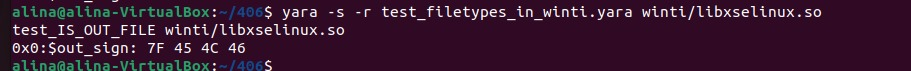
\includegraphics[width=\textwidth]{file_ver.jpg}
    \caption{Classifying the file of malware}
    \label{fig:file_type}
    
\end{figure}




